\documentclass[11pt]{article}
\usepackage[margin=0.82in]{geometry}
\usepackage{amsmath,amssymb,amsthm}
\usepackage{graphicx}
\setlength{\parindent}{0pt}
\setlength{\parskip}{0.55em}

\newtheorem{theorem}{Theorem}
\newcommand{\R}{\mathbb R}
\newcommand{\T}{\mathcal T}
\newcommand{\Dop}{D_+}

\title{Failure of the proposed endpoint H\"older inequality\\
\large A counterexample to arXiv:1906.10772, Open Question (ii)}
\author{Run \texttt{fa\_banach\_001} --- \texttt{agent\_lane\_03}}
\date{12 August 2026}

\begin{document}
\maketitle

\textbf{Status.} High-confidence candidate counterexample, pending human
review.  The construction gives a complete negative answer to Open Question
(ii) as literally stated; no claim is made about questions (i) or (iii).

\section*{Source conjecture}

Miana and Oliva-Maza, \emph{Generalized Stieltjes and other integral
operators on Sobolev--Lebesgue spaces}, arXiv:1906.10772, conjecture that
whenever $1/r=1/p+1/q$ with $p,q,r\in[1,\infty]$, pointwise multiplication
satisfies
\begin{equation}
 \|fg\|_{\alpha,r}
 \le C_\alpha\|f\|_{\alpha,p}\|g\|_{\alpha,q}. \tag{H}
\end{equation}
Crucially, the displayed range includes $p=\infty$.  Their Remark 3.1
proposes
\[
 \|f\|_{\alpha,\infty}
 =\frac1{\Gamma(\alpha+1)}
   \operatorname*{ess\,sup}_{t>0}t^\alpha|W_+^\alpha f(t)|,
\]
and explicitly observes that this need not control $\|f\|_\infty$.

\begin{center}
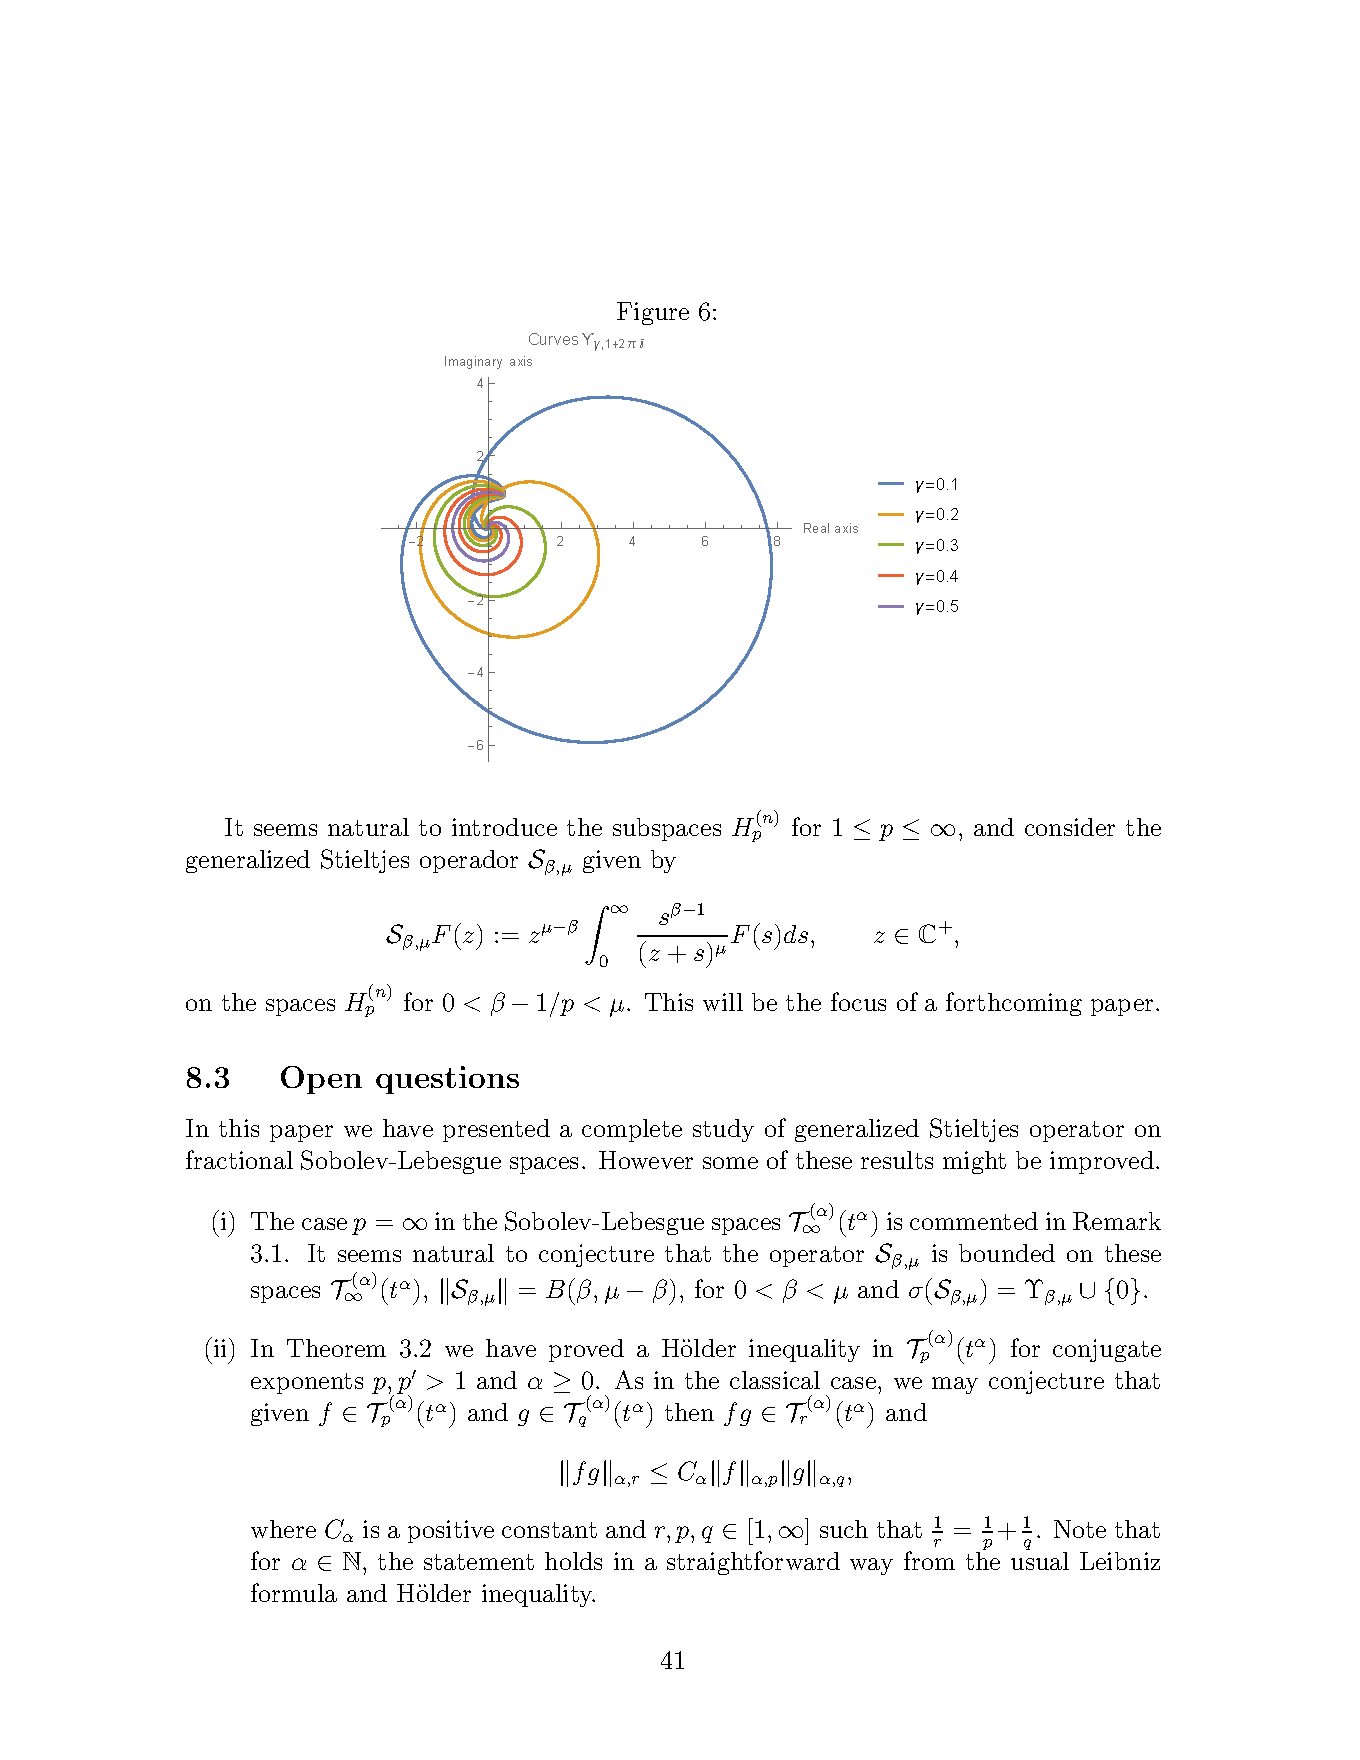
\includegraphics[width=0.90\textwidth,trim=0 30 0 395,clip]{figures/open_questions_page_41.png}
\end{center}

\section*{The counterexample}

At $\alpha=1$, one has $W_+^1f=-f'$ and $\Gamma(2)=1$, hence
\[
 \|f\|_{1,s}=\|-t f'(t)\|_{L^s(0,\infty)}quad(1\le s<\infty),
 \qquad
 \|f\|_{1,\infty}=\operatorname*{ess\,sup}_{t>0}t|f'(t)|.
\]
For finite $s$, the source proves that $\Dop^1 f=-tf'$ is an isometry from
$\T_s^{(1)}(t)$ onto $L^s(0,\infty)$, with inverse
\begin{equation}
 ((\Dop^1)^{-1}h)(t)=\int_t^\infty \frac{h(s)}s\,ds. \tag{1}
\end{equation}

\begin{theorem}
For every $q\in(1,\infty)$, multiplication does not map
\[
 \T_\infty^{(1)}(t)\times\T_q^{(1)}(t)
 \longrightarrow\T_q^{(1)}(t)
\]
under either the maximal finite-norm interpretation of the first space or
the natural completion of the Schwartz core.  Consequently (H) is false
with $\alpha=1$, $p=\infty$, and $r=q$.
\end{theorem}

\begin{proof}
Choose $a\in(0,1)$ and put $b=a+1/q$.  Let
$\eta\in C_c^\infty([0,\infty))$ equal $1$ on $(0,1/4)$ and $0$ on
$(1/2,\infty)$.  With $L(t)=\log(e/t)$, define for $t>0$
\[
 f(t)=\eta(t)L(t)^a,
 \qquad
 g(t)=\eta(t)t^{-1/q}L(t)^{-b}.
\]
On $(0,1/4)$,
\begin{equation}
 -t f'(t)=aL(t)^{a-1}\longrightarrow0,
 \qquad
 -t g'(t)=\left(\frac1q-\frac b{L(t)}\right)g(t). \tag{2}
\end{equation}
The cutoff terms are bounded and compactly supported away from zero.
Therefore $h_f=-tf'$ extends continuously to $0$ with value $0$ and is
bounded with compact support.  It can be approximated uniformly by functions
$h_{f,n}\in C_c^\infty(0,\infty)$.  Formula (1) gives
$f_n=(\Dop^1)^{-1}h_{f,n}$ in the Schwartz core and
$\|f_n-f\|_{1,\infty}=\|h_{f,n}-h_f\|_\infty\to0$.  Thus $f$ belongs even
to the completion interpretation of $\T_\infty^{(1)}(t)$.

Next,
\[
 \int_0^{1/4}|g(t)|^qdt
 =\int_0^{1/4}\frac{dt}{tL(t)^{bq}}<\infty,
 \qquad bq=aq+1>1.
\]
Equation (2) shows that $h_g=-tg'\in L^q(0,\infty)$.  Approximating $h_g$
in $L^q$ by $C_c^\infty(0,\infty)$ and applying (1) proves
$g\in\T_q^{(1)}(t)$.

But on $(0,1/4)$ the choice $b=a+1/q$ gives
\[
 |f(t)g(t)|^q
 =t^{-1}L(t)^{q(a-b)}
 =\frac1{tL(t)}.
\]
Hence
\[
 \int_0^{1/4}|f(t)g(t)|^qdt
 =\int_0^{1/4}\frac{dt}{t\log(e/t)}=\infty.
\]
The source's continuous inclusion $\T_q^{(1)}(t)\hookrightarrow L^q$
therefore implies $fg\notin\T_q^{(1)}(t)$.
\end{proof}

\section*{Why the stated integer-order argument misses this}

For finite exponents, the usual Leibniz rule and H\"older inequality do
indeed give the integer-order claim.  At $p=\infty$, however, the proposed
norm controls $tf'$ but not $f$.  The first Leibniz term $f\,tg'$ is thus
uncontrolled.  The source already flags this defect by noting that
$\log(1+t)$ has finite $\|\cdot\|_{1,\infty}$ norm but is unbounded; the
construction above localizes the same phenomenon at zero so that it remains
inside the Schwartz-core completion.

A precise repair is immediate: if the endpoint norm is strengthened to
$\|f\|_\infty+\|f\|_{1,\infty}$, then
\begin{align*}
 \|fg\|_{1,q}
 &\le \|f\|_\infty\|g\|_{1,q}
      +\|f\|_{1,\infty}\|g\|_{L^q}\\
 &\le C\bigl(\|f\|_\infty+\|f\|_{1,\infty}\bigr)\|g\|_{1,q}.
\end{align*}
Thus the failure is exactly the absent $L^\infty$ control, not an exotic
fractional-calculus effect.

\section*{Proof intuition and scope}

The weight $t$ makes logarithmic singularities cheap: $L(t)^a$ diverges at
zero, while $t|(L^a)'|=aL^{a-1}\to0$ for $a<1$.  The second factor is placed
just inside $L^q$ by a logarithmic power.  Multiplication consumes exactly
that logarithmic margin and creates the borderline divergent density
$dt/(t\log(e/t))$.

This fully refutes Open Question (ii) in its stated exponent range.  It does
not decide whether a finite-exponent version holds for noninteger $\alpha$,
nor does it address the Stieltjes boundedness/spectrum conjecture (i) or the
informal representation conjecture (iii).  Exact-ID, title, core-keyword,
and official-arXiv searches through 12 August 2026 found no later matching
counterexample; this is a bounded novelty audit, not a priority claim.

{\small
\textbf{Reference.}
P.~J. Miana and J. Oliva-Maza, \emph{Generalized Stieltjes and other integral
operators on Sobolev--Lebesgue spaces}, arXiv:1906.10772, Remark 3.1 and
Open Question (ii).
}

\end{document}
